\documentclass{standalone}
%
\usepackage{tikz}
\usetikzlibrary{backgrounds,shapes.callouts}
\usepackage{tkz-euclide}
\usepackage{xcolor}
%\usepackage{pgfplots}
%\usepackage{freetikz}
%\usetikzlibrary{shapes}
%\definecolor{eduinafred}{HTML}{BB2D58}
%\definecolor{eduinafblu}{HTML}{1D71B8}
%
\definecolor{space}{HTML}{0A2543}
\definecolor{mercury}{HTML}{846549}
\definecolor{venus}{HTML}{BB9765}
\definecolor{earth}{HTML}{0089FA}
\definecolor{mars}{HTML}{DC7B4E}
\definecolor{jupiter}{HTML}{A79476}
\definecolor{saturn}{HTML}{DBBD9B}
\definecolor{saturnring}{HTML}{857C73}
\definecolor{uranus}{HTML}{b1d8dd}
\definecolor{neptune}{HTML}{799bc1}
\definecolor{pluto}{HTML}{ceaa8a}
\definecolor{dida}{HTML}{FFDE00}
\definecolor{title}{HTML}{FBA706}
%
%\definecolor{glasses}{HTML}{08663D}
\definecolor{moon}{HTML}{AFAFAF}
%\definecolor{craterm}{HTML}{616060}
%\definecolor{linem}{HTML}{DBDBDB}
%\definecolor{core3}{HTML}{FFD016}
%
\usepackage{fontspec}
\setmainfont{Open Dyslexic}
%\setmainfont{Montserrat Medium}
%
\title{Sistema Solare}
\begin{document}
	\tikzset{
		partial ellipse/.style args = {#1:#2:#3}{insert path={+ (#1:#3) arc (#1:#2:#3)}},
		notice/.style  = { draw, ellipse callout, callout relative pointer={#1} },
	}
	\begin{tikzpicture}[background rectangle/.style={fill=white},show background rectangle,>={[inset=0,angle'=27]Stealth}]
		\def\rsun{1}
		\def\rmer{0.2}
		\def\rven{0.5}
		\def\ret{0.53}
		\def\rmn{0.2}
		\def\rms{0.28}
		\def\rj{1}
		\def\rsat{1}
		\def\rur{1}
		\def\rnp{1}
		\def\rp{0.1}
		%
		\def\d{3}
		%
		\draw [use as bounding box] (-20,20) -| (20,20) |- (20,-100) -| (-20,-100);
		%title
		\begin{scope}
			\draw [black,ultra thick,fill=title] (-18,18.5) rectangle (18,11.5);
			\node (example-textwidth-2) [align=center, text width=40cm, color=black, font=\fontsize{90pt}{91pt}\selectfont] at (0,15) {Il sistema tolemaico};
		\end{scope}
		%
		\begin{scope}[shift={(-10,7)}]
			\node at (23,0) {
\includegraphics[width=5cm]{img/carl_sagan}};
			\node (example-textwidth-2) [notice={(3,0.5)}, ultra thick, right, align=center, text width=12cm, color=black, fill=white, font=\fontsize{23pt}{24pt}\selectfont] at (1,-1) {Il modello geocentrico risale ad \textbf{Apollonio di Perga} e venne successivamente perfezionato da \textbf{Ipparco}. I loro lavori, pero', ci sono giunti in maniera indiretta tramite l'\emph{Almagesto} di \textbf{Tolomeo}.};
		\end{scope}
		%
		\begin{scope}[shift={(-15,-5)}]
			\node at (5,0) {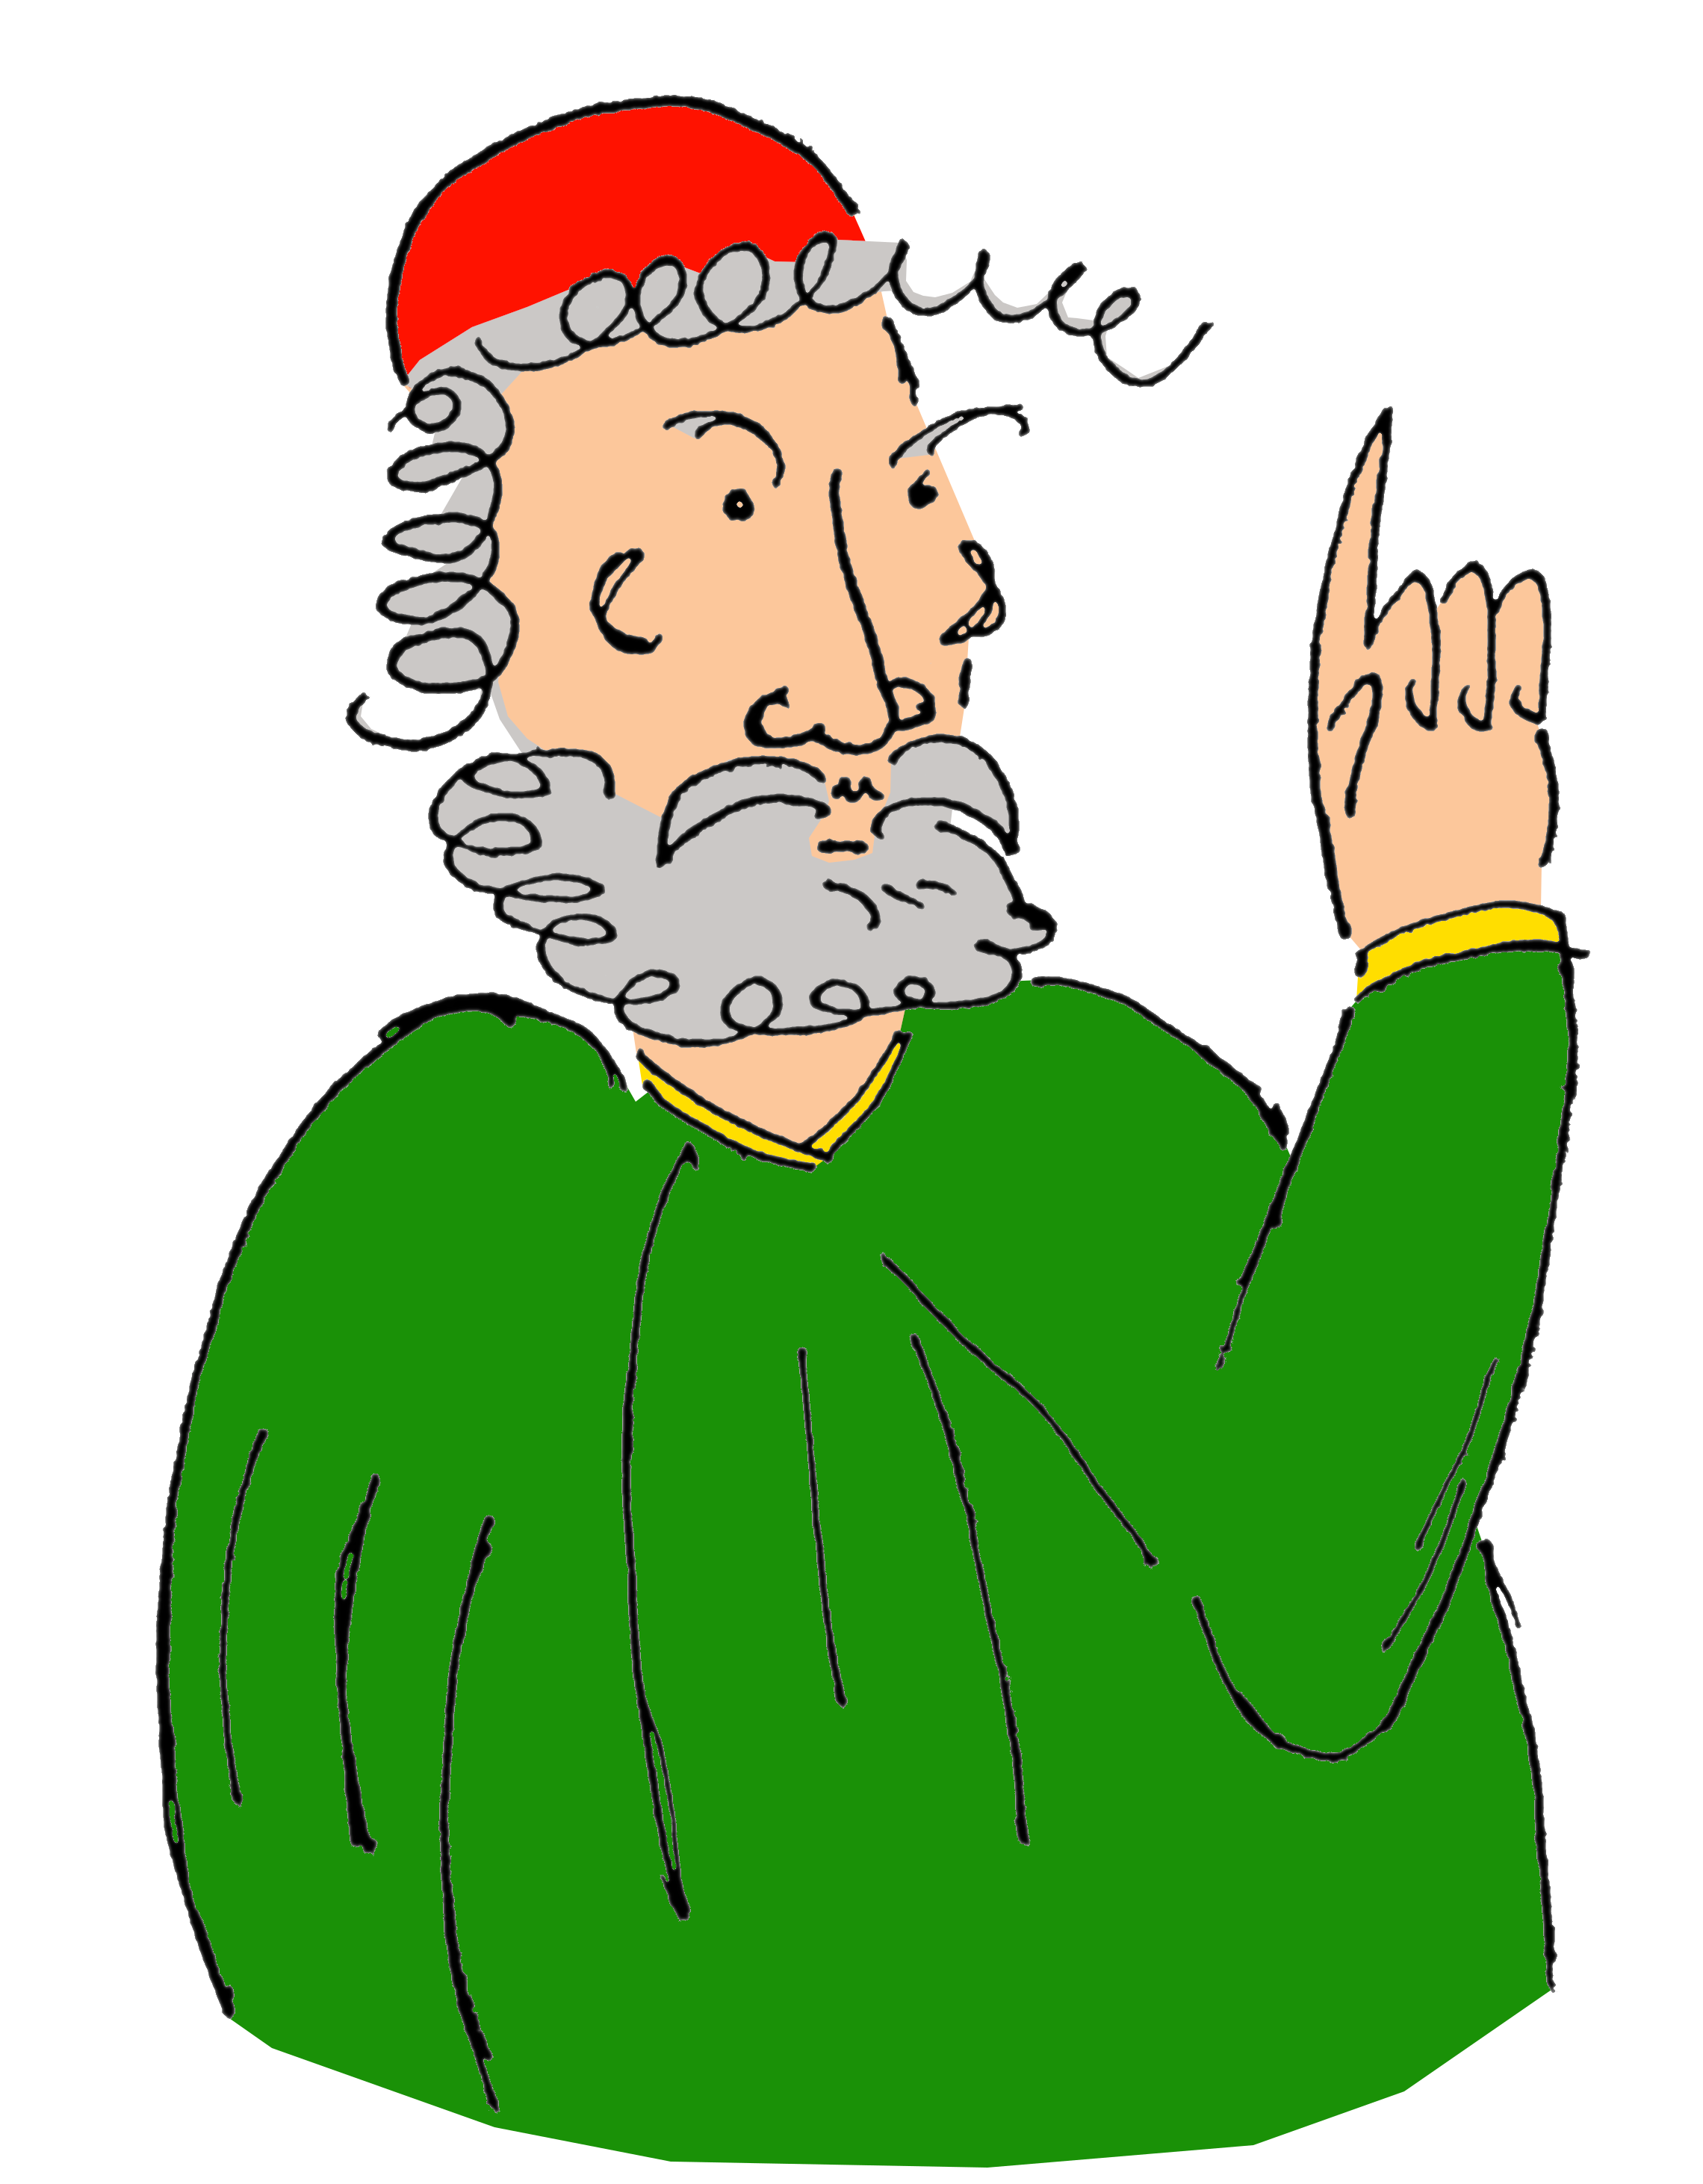
\includegraphics[width=8cm]{img/tolomeo}};
			\node (example-textwidth-2) [notice={(-3,-1)}, ultra thick, right, align=center, text width=12cm, color=black, fill=white, font=\fontsize{23pt}{24pt}\selectfont] at (8,4.5) {Finalmente si parla di me!};
			\node (example-textwidth-2) [notice={(3,1)}, ultra thick, right, align=center, text width=12cm, color=black, fill=white, font=\fontsize{23pt}{24pt}\selectfont] at (8,0) {Tolomeo! Non interrompere!};
			\node (example-textwidth-2) [notice={(-3,1)}, ultra thick, right, align=center, text width=12cm, color=black, fill=white, font=\fontsize{23pt}{24pt}\selectfont] at (8,-4.5) {Ma... Signora maestra! Sono io il protagonista!};
		\end{scope}
		%
		\begin{scope}[shift={(-15,-14)}]
			\draw [fill=dida, ultra thick] (1,2) rectangle (30.5,-2);
			\node at (2,0) {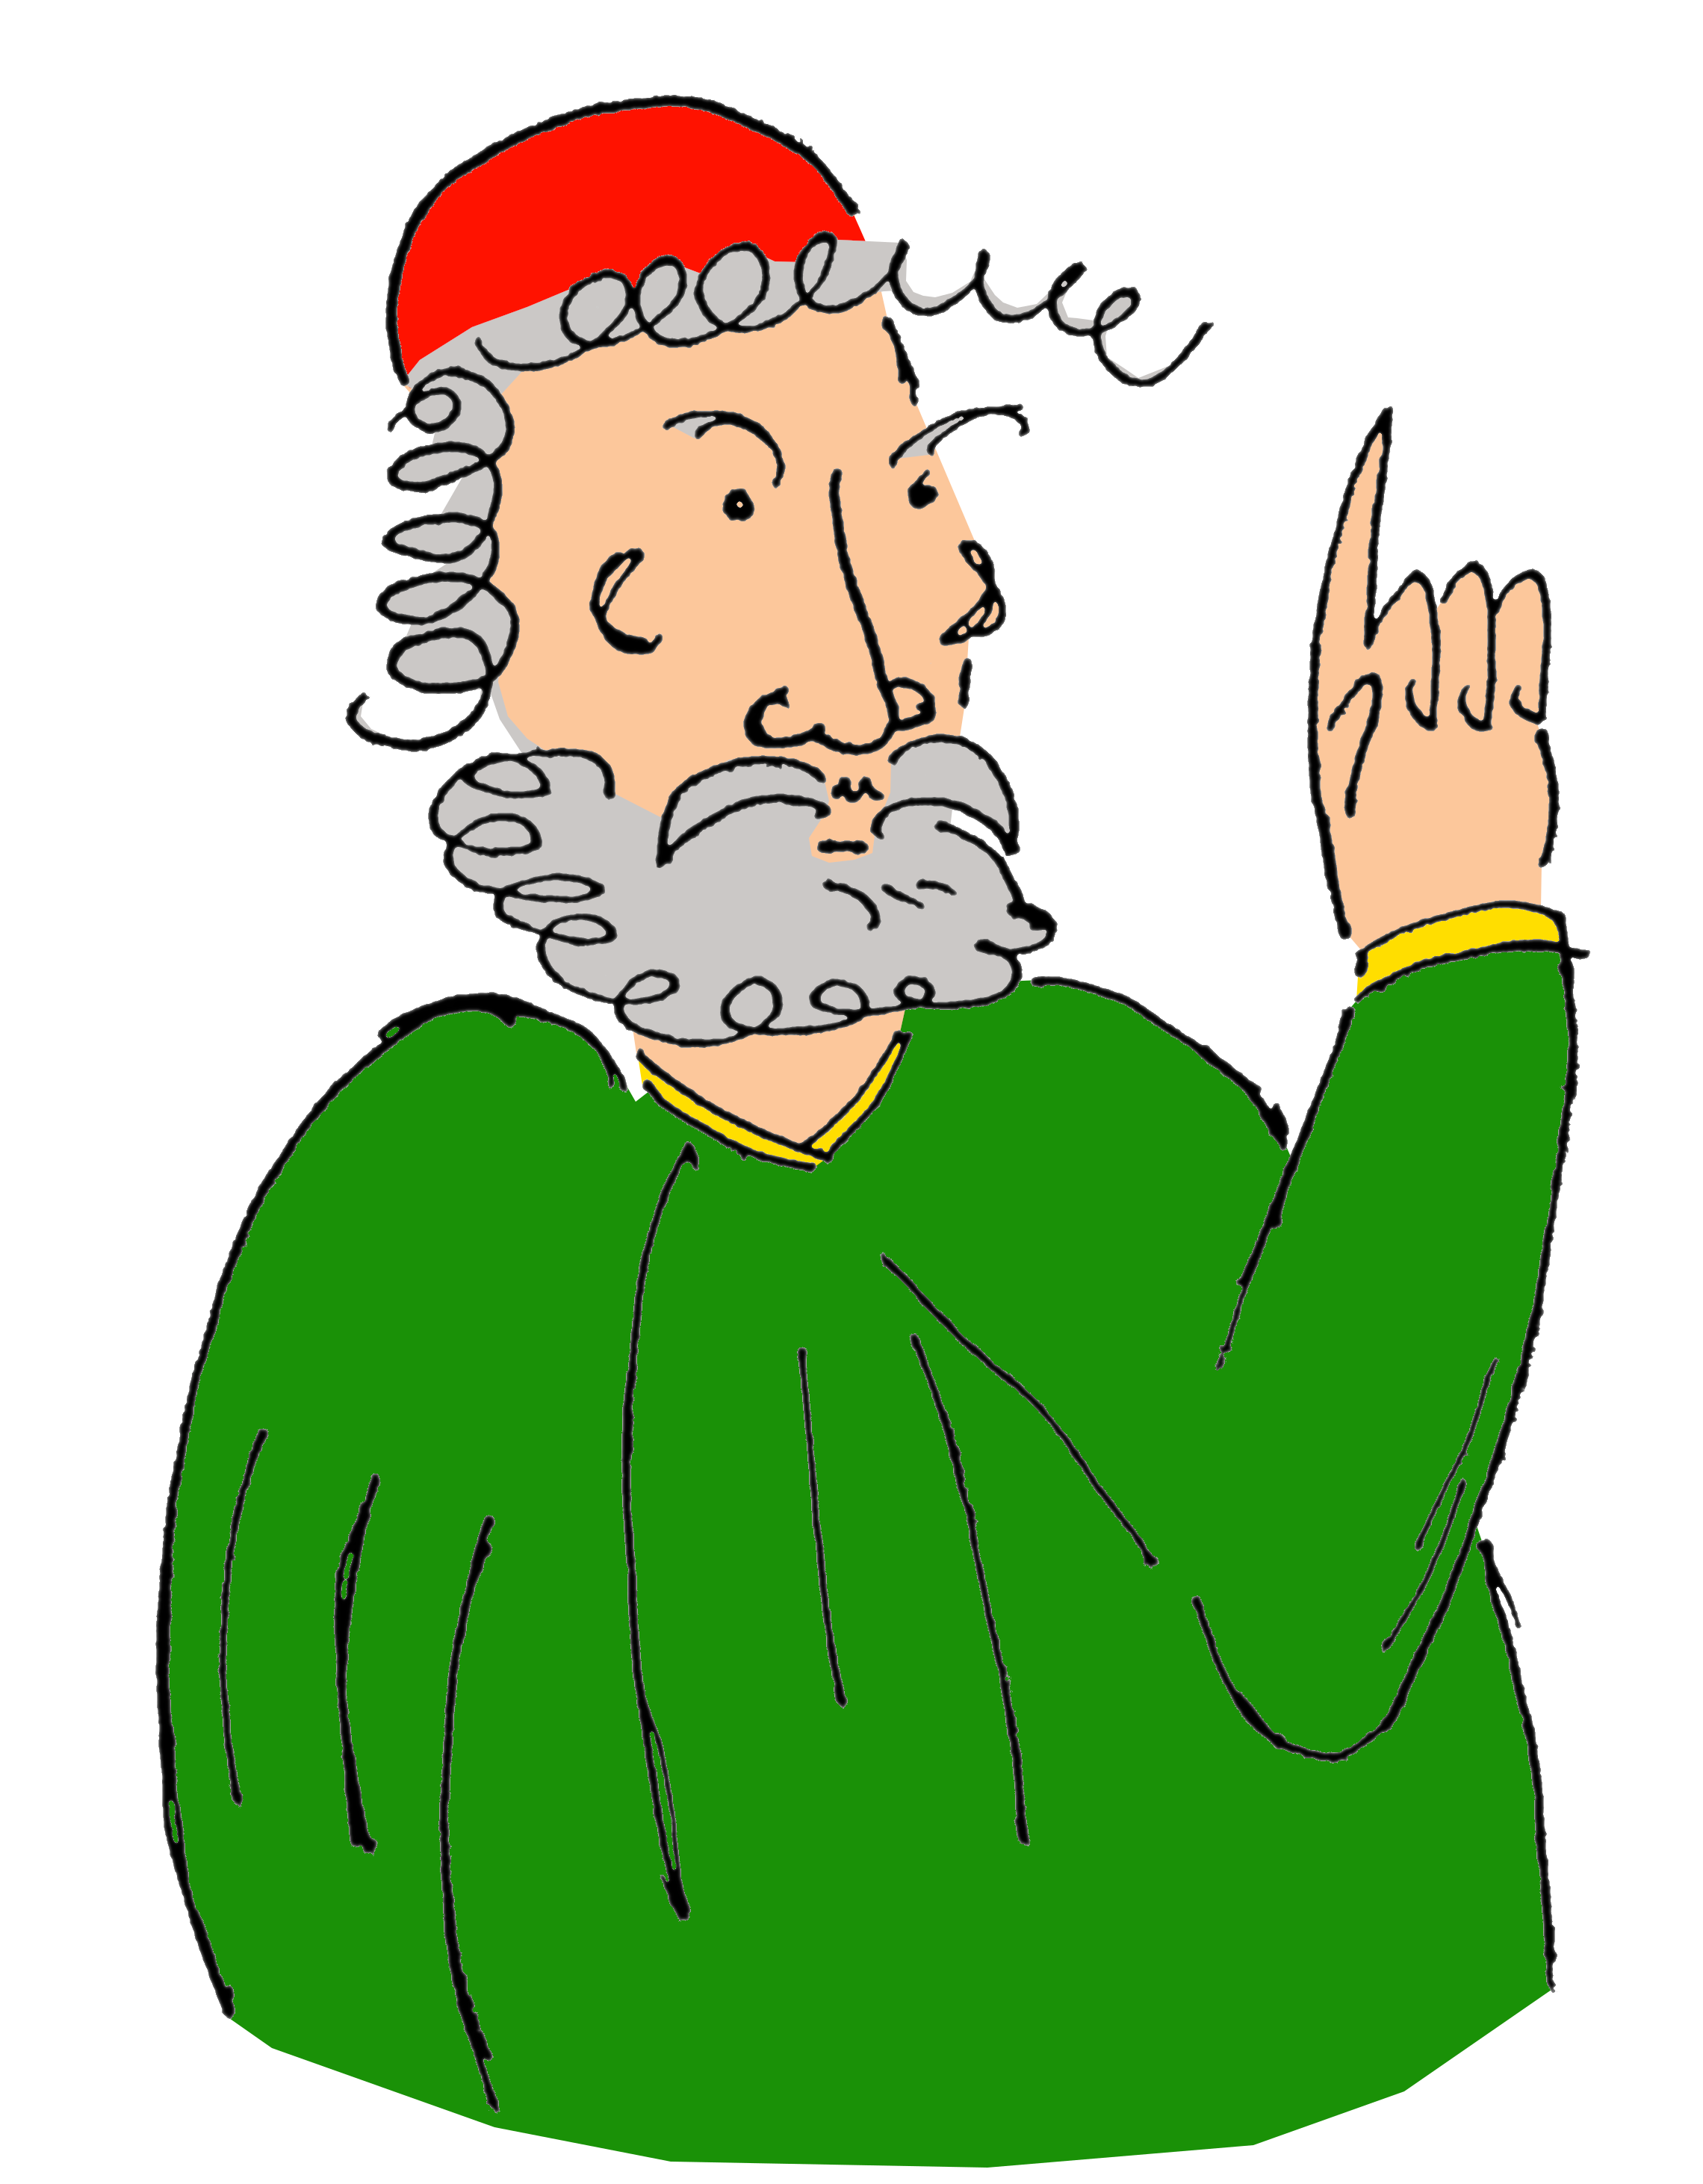
\includegraphics[width=4cm]{img/tolomeo}};
			\node (example-textwidth-2) [right, align=left, text width=26cm, color=black, font=\fontsize{23pt}{24pt}\selectfont] at (4.5,0) {All'epoca pensavamo, per molti motivi, che la Terra fosse al centro dell'Universo. Quindi mi misi a fare i calcoli per rendere il modello compatibile con le osservazioni: nascono cosi' gli epicicli.};
		\end{scope}
		%
		\begin{scope}[shift={(-3,-30)}]
			\draw [fill=space] (-14,13) rectangle (18,-7);
			\tkzDefPoint(-6,0){E} %Earth
			\tkzDefShiftPoint[E](\d,0){L0} %Moon
			\tkzDefPointBy[rotation= center E angle 120](L0) \tkzGetPoint{L}
			\tkzDefShiftPoint[E](2*\d,0){H0} %Mercury
			\tkzDefPointBy[rotation= center E angle 15](H0) \tkzGetPoint{Hc}
			\tkzDefShiftPoint[E](3*\d,0){H1}
			\tkzDefPointBy[rotation= center E angle 15](H1) \tkzGetPoint{Hr}
			\tkzDefPointBy[rotation= center E angle 15](H1) \tkzGetPoint{H2}
			\tkzDefPointBy[rotation= center Hc angle 60](H2) \tkzGetPoint{H}
			\tkzDefShiftPoint[E](5*\d,0){V0} %Venus
			\tkzDefPointBy[rotation= center E angle 15](V0) \tkzGetPoint{Vc}
			\tkzDefShiftPoint[E](7 * \d,0){S0} %Sun
			\tkzDefPointBy[rotation= center E angle 15](S0) \tkzGetPoint{S}
			\tkzDefPointBy[rotation= center Vc angle -75](S) \tkzGetPoint{V}
			%
			\tkzDrawCircle[color=moon,ultra thick](E,L)
			%
			\tkzDrawCircle[color=mercury,ultra thick](Hc,Hr)
			\tkzDrawSegment[color=mercury,ultra thick](Hc,H)
			\tkzDrawCircle[color=mercury,ultra thick](E,Hc)
			%
			\tkzDrawCircle[color=venus,ultra thick](Vc,S)
			\tkzDrawSegment[color=venus, ultra thick](Vc,V)
			\tkzDrawArc[color=venus,ultra thick,rotate](E,Vc)(30)
			\tkzDrawArc[color=venus,ultra thick,rotate](E,Vc)(-30)
			%
			\tkzDrawSegment[color=white,ultra thick](E,S)
			\tkzDrawArc[ultra thick, color=white, rotate](E,S)(30)
			\tkzDrawArc[ultra thick, color=white, rotate](E,S)(-30)
			\tkzDefShiftPoint[E](0:\ret){E1}
			\tkzDrawCircle[color=black,ultra thick,fill=earth](E,E1)
			\node [above, xshift=3cm, text width=10cm, color=white, font=\fontsize{15pt}{16pt}\selectfont] at (E) {Terra};
			\tkzDefShiftPoint[L](0:\rmn){L1}
			\tkzDrawCircle[color=black,ultra thick,fill=moon](L,L1)
			\node [above, xshift=3cm, text width=10cm, color=white, font=\fontsize{15pt}{16pt}\selectfont] at (L) {Luna};
			\tkzDefShiftPoint[H](0:\rmer){H1}
			\tkzDrawCircle[color=black,ultra thick,fill=mercury](H,H1)
			\node [above, xshift=3.5cm, yshift=0.5cm, text width=10cm, color=white, font=\fontsize{15pt}{16pt}\selectfont] at (H) {Mercurio};
			\tkzDefShiftPoint[V](0:\rven){V1}
			\tkzDrawCircle[color=black,ultra thick,fill=venus](V,V1)
			\node [below, xshift=5.5cm, text width=10cm, color=white, font=\fontsize{15pt}{16pt}\selectfont] at (V) {Venere};
			\tkzDefShiftPoint[S](0:\ret){S1}
			\tkzDrawCircle[color=black,ultra thick,fill=white](S,S1)
			\node [above, xshift=6.5cm, text width=10cm, color=white, font=\fontsize{15pt}{16pt}\selectfont] at (S) {Sole};
			%
			\node [yshift=0.5cm, text width=10cm, color=mercury, font=\fontsize{15pt}{16pt}\selectfont] at (0,2*\d) {deferente};
			\node [text width=10cm, color=mercury, font=\fontsize{15pt}{16pt}\selectfont] at (1.9*\d,-0.6*\d) {epiciclo};
			\draw [black,ultra thick] (-14,13) rectangle (18,-7);
		\end{scope}
		%
		\begin{scope}[shift={(-10,-42)}]
			\node at (23,0) {
\includegraphics[width=5cm]{img/carl_sagan}};
			\node (example-textwidth-2) [notice={(3,0.5)}, ultra thick, right, align=center, text width=12cm, color=black, fill=white, font=\fontsize{23pt}{24pt}\selectfont] at (1,-1) {Epicicli che, in realta', aveva gia' introdotto Apollonio.};
			\node at (-2,-2) {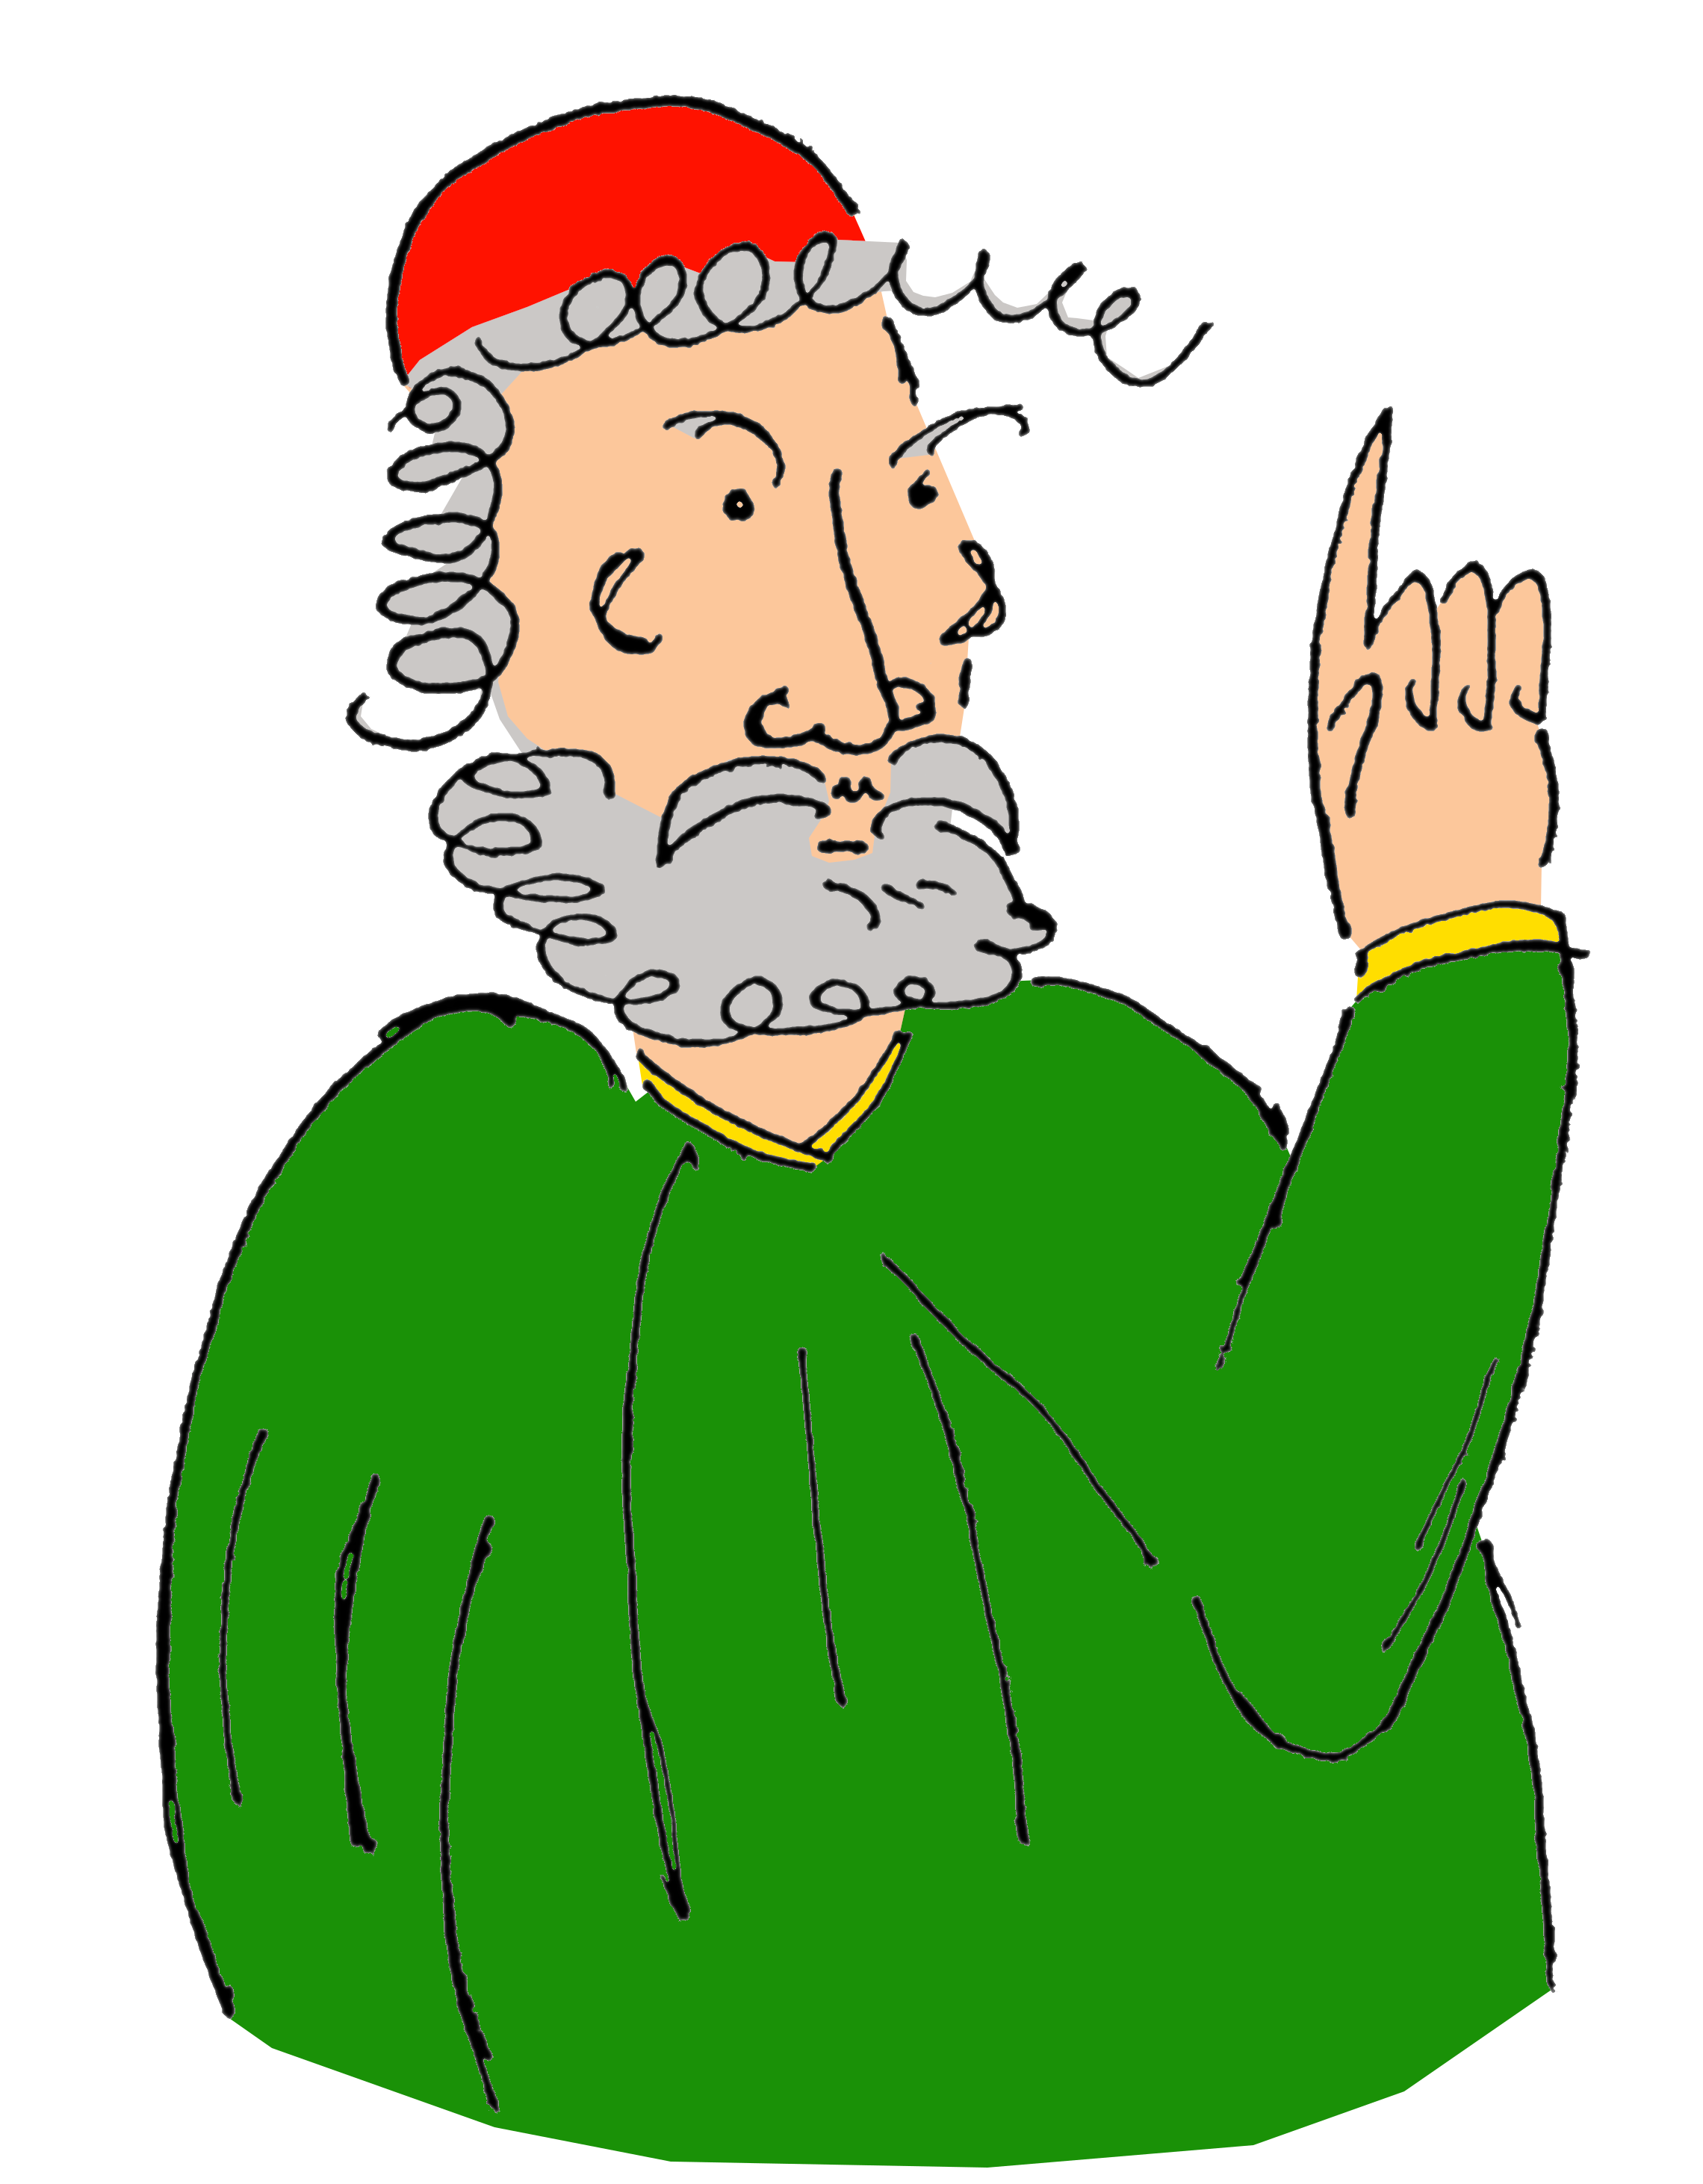
\includegraphics[width=6cm]{img/tolomeo}};
			\node (example-textwidth-2) [notice={(-3,1)}, ultra thick, right, align=center, text width=5cm, color=black, fill=white, font=\fontsize{23pt}{24pt}\selectfont] at (0,-4.5) {Dettagli!};
		\end{scope}
		%
		\begin{scope}[shift={(-10,-51)}]
			\node at (0,-2) {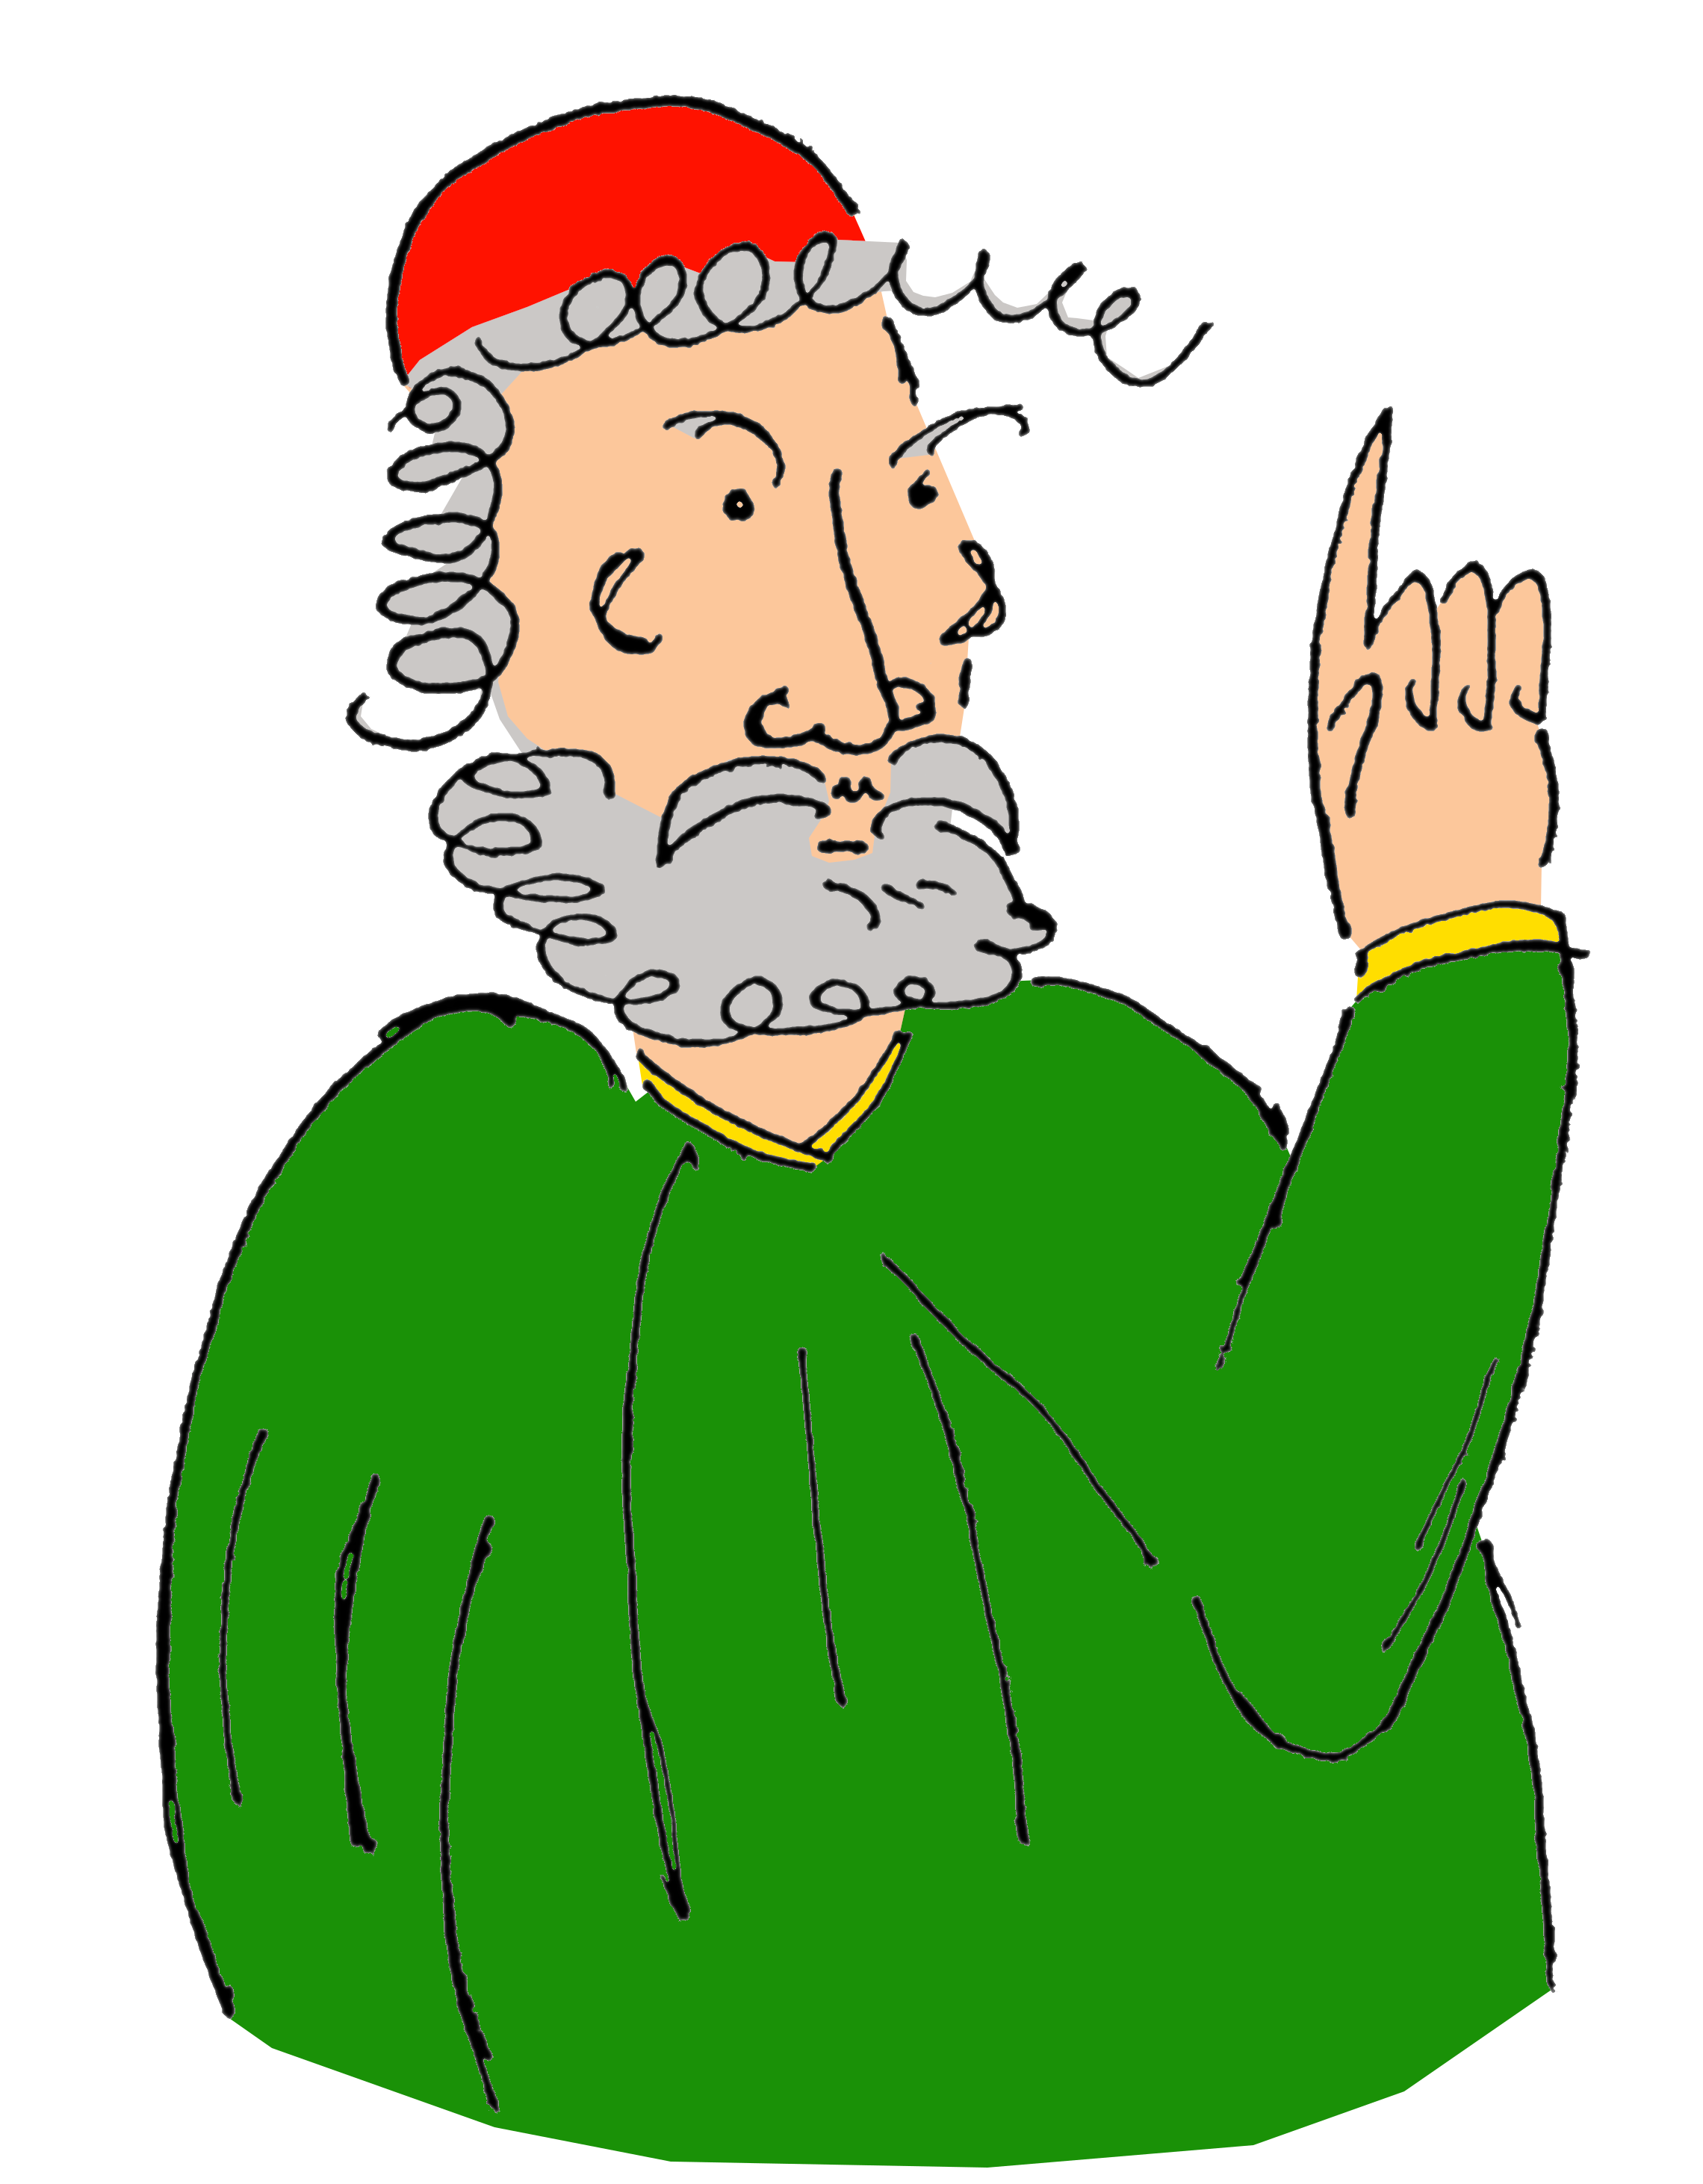
\includegraphics[width=6cm]{img/tolomeo}};
			\node (example-textwidth-2) [notice={(-3,1)}, ultra thick, right, align=center, text width=12cm, color=black, fill=white, font=\fontsize{23pt}{24pt}\selectfont] at (2,-4.5) {Cio' che conta e' che il mio modello era piu' preciso di quello di Aristarco!};
		\end{scope}
		%
		\begin{scope}[shift={(-3,-73)}]
			\draw [fill=space] (-14,15) rectangle (20,-15);
			\tkzDefPoint(-6,0){E} %Earth
			\tkzDefShiftPoint[E](\d,0){S0} %Sun
			\tkzDefPointBy[rotation= center E angle 15](S0) \tkzGetPoint{S}
			\tkzDefShiftPoint[E](2*\d,0){M0} %Mars
			\tkzDefPointBy[rotation= center E angle 45](M0) \tkzGetPoint{Mc}
			\tkzDefShiftPoint[Mc](\d,0){Mr}
			\tkzDefPointBy[rotation= center Mc angle 15](Mr) \tkzGetPoint{M}
			\tkzDefShiftPoint[E](4*\d,0){J0} %Jupiter
			\tkzDefPointBy[rotation= center E angle -30](J0) \tkzGetPoint{Jc}
			\tkzDefShiftPoint[Jc](\d,0){Jr}
			\tkzDefPointBy[rotation= center Jc angle 15](Jr) \tkzGetPoint{J}
			\tkzDefShiftPoint[E](6*\d,0){R0} %Saturn
			\tkzDefPointBy[rotation= center E angle 30](R0) \tkzGetPoint{Rc}
			\tkzDefShiftPoint[Rc](\d,0){Rr}
			\tkzDefPointBy[rotation= center Rc angle 15](Rr) \tkzGetPoint{R}
			\tkzDefShiftPoint[E](8*\d,0){St} %Fixed stars
			%
			\tkzDrawSegment[color=white,ultra thick](E,S)
			\tkzDrawCircle[color=white,ultra thick](E,S)
			\tkzDrawCircle[color=mars,ultra thick](Mc,Mr)
			\tkzDrawSegment[color=mars,ultra thick](Mc,M)
			\tkzDrawCircle[color=mars,ultra thick](E,Mc)
			\tkzDrawCircle[color=jupiter,ultra thick](Jc,Jr)
			\tkzDrawSegment[color=jupiter,ultra thick](Jc,J)
			\tkzDrawArc[color=jupiter,ultra thick,rotate](E,Jc)(100)
			\tkzDrawArc[color=jupiter,ultra thick,rotate](E,Jc)(-60)
			\tkzDrawCircle[color=saturn,ultra thick](Rc,Rr)
			\tkzDrawSegment[color=saturn,ultra thick](Rc,R)
			\tkzDrawArc[color=saturn,ultra thick,rotate](E,Rc)(20)
			\tkzDrawArc[color=saturn,ultra thick,rotate](E,Rc)(-80)
			\tkzDrawArc[color=white,ultra thick,rotate](E,St)(40)
			\tkzDrawArc[color=white,ultra thick,rotate](E,St)(-40)
			%
			\tkzDefShiftPoint[E](0:\ret){E1}
			\tkzDrawCircle[color=black,ultra thick,fill=earth](E,E1)
			\node [above, xshift=3cm, text width=10cm, color=white, font=\fontsize{15pt}{16pt}\selectfont] at (E) {Terra};
			\tkzDefShiftPoint[S](0:\ret){S1}
			\tkzDrawCircle[color=black,ultra thick,fill=white](S,S1)
			\node [above, xshift=6.5cm, text width=10cm, color=white, font=\fontsize{15pt}{16pt}\selectfont] at (S) {Sole};
			\tkzDefShiftPoint[M](0:\ret){M1}
			\tkzDrawCircle[color=black,ultra thick,fill=mars](M,M1)
			\node [above, xshift=6.5cm, text width=10cm, color=white, font=\fontsize{15pt}{16pt}\selectfont] at (M) {Marte};
			\tkzDefShiftPoint[J](0:\ret){J1}
			\tkzDrawCircle[color=black,ultra thick,fill=jupiter](J,J1)
			\node [above, xshift=6.5cm, text width=10cm, color=white, font=\fontsize{15pt}{16pt}\selectfont] at (J) {Giove};
			\tkzDefShiftPoint[R](0:\ret){R1}
			\tkzDrawCircle[color=black,ultra thick,fill=saturn](R,R1)
			\node [above, xshift=6cm, text width=10cm, color=white, font=\fontsize{15pt}{16pt}\selectfont] at (R) {Saturno};
			\node [above, xshift=2cm, text width=4cm, color=white, font=\fontsize{15pt}{16pt}\selectfont] at (5.5*\d,9) {Stelle fisse};
			\draw [color=black,ultra thick] (-14,15) rectangle (20,-15);
		\end{scope}
		%
		\begin{scope}[shift={(-10,-92)}]
			\node at (23,0) {
\includegraphics[width=5cm]{img/carl_sagan}};
			\node (example-textwidth-2) [notice={(3,0.5)}, ultra thick, right, align=center, text width=12cm, color=black, fill=white, font=\fontsize{23pt}{24pt}\selectfont] at (1,-1) {Questo perche' non erano ancora arrivati \textbf{Tycho Brahe}, \textbf{Johannes Kepler}, \textbf{Nicolaus Copernicus} e \textbf{Galileo Galilei}.};
		\end{scope}
		%
		\begin{scope}[shift={(-10,-98)}]
			\node at (27,0) () {
\includegraphics[width=3.7cm]{img/licenza}};
			\node at (18,-0.1) {\textcolor{black}{\fontsize{14}{15}\selectfont Testo e illustrazioni: @ulaulaman - Gianluigi Filippelli}};
		\end{scope}
	\end{tikzpicture}
%
\end{document}